\chapter{Magnetické převodovky}

Jak jsme v předchozí kapitole ukázali, přenášení momentu pomocí magnetů je možné a dokonce poměrně dobře prozkoumané. První patenty o přenosu momentu síly pomocí magnetů se objevily již na začátku 20. století \cite{patent}, ale kvůli technologickým nedostatkům doby byly brzy opuštěny. Teprve v posledních letech se díky pokrokům ve vědě opět objevuje zájem o magnetické převodovky.

% Výhody
Magnetické převodovky byly dříve zavrhnuty kvůli mnohým nedostatkům:

\begin{enumerate}[topsep=0pt, partopsep=0pt]
    \setlength{\itemsep}{0pt}%
    \setlength{\parskip}{0pt}%
    \item Maximální přenositelný moment síly je malý.
    \item Složitá konstrukce.
    \item Potřeba silných magnetických materiálů a materiálů s vysokou permeabilitou.
    \item Nedostatek využití, kde by mechanické převody nefungovaly lépe.
\end{enumerate}

V dnešní době se však objevují nové situace, ve kterých jsou magnetické převodovky dobrým řešením. Jako příklad uvedeme jejich použití ve vesmíru. Magnetické převodovky totiž dobře odolávají nízkým teplotám \cite{NASA_MG} narozdíl od standardních lubrikačních látek, které jsou potřebné k běhu mechanických převodů. Nejvýznamnějšími výhodami magnetickým převodovek jsou:

\begin{enumerate}[topsep=0pt, partopsep=0pt]
    \setlength{\itemsep}{0pt}%
    \setlength{\parskip}{0pt}%
    \item Srovnatelná objemová hustota momentu síly magnetických a mechanických převodovek \cite{torque_dens}.
    \item Využití, ve kterých mechanické převodovky nemohou být použity.
    \item Minimální tepelné ztráty.
    \item Nízká či nulová údržba a možnost používání bez lubrikace.
    \item Automatická ochrana proti přetížení.
    \item Kompaktnost a možnost slučovat více magnetických systémů do jednoho celku \cite{MT_full}.
    \item Možnost nahradit mnohé druhy mechanických převodů.
    \item Odolnost proti písku a jiným nečistotám.
    \item Možnost použití ve vakuu bez potřeby odplynění maziv.
\end{enumerate}

\clearpage

\begin{wrapfigure}{r}{0.50\textwidth}
    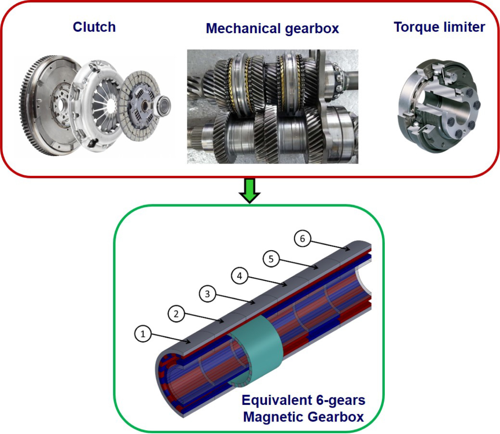
\includegraphics[width=0.45\textwidth]{magnetic_transmission.png}
    \centering
    \caption[Nákres šestistupňové magnetické převodovky]{Nákres šestistupňové magnetické převodovky (zdroj: \cite{MT_full}).}
    \label{fig:magnetic_transmission}

    \vspace{1cm}

    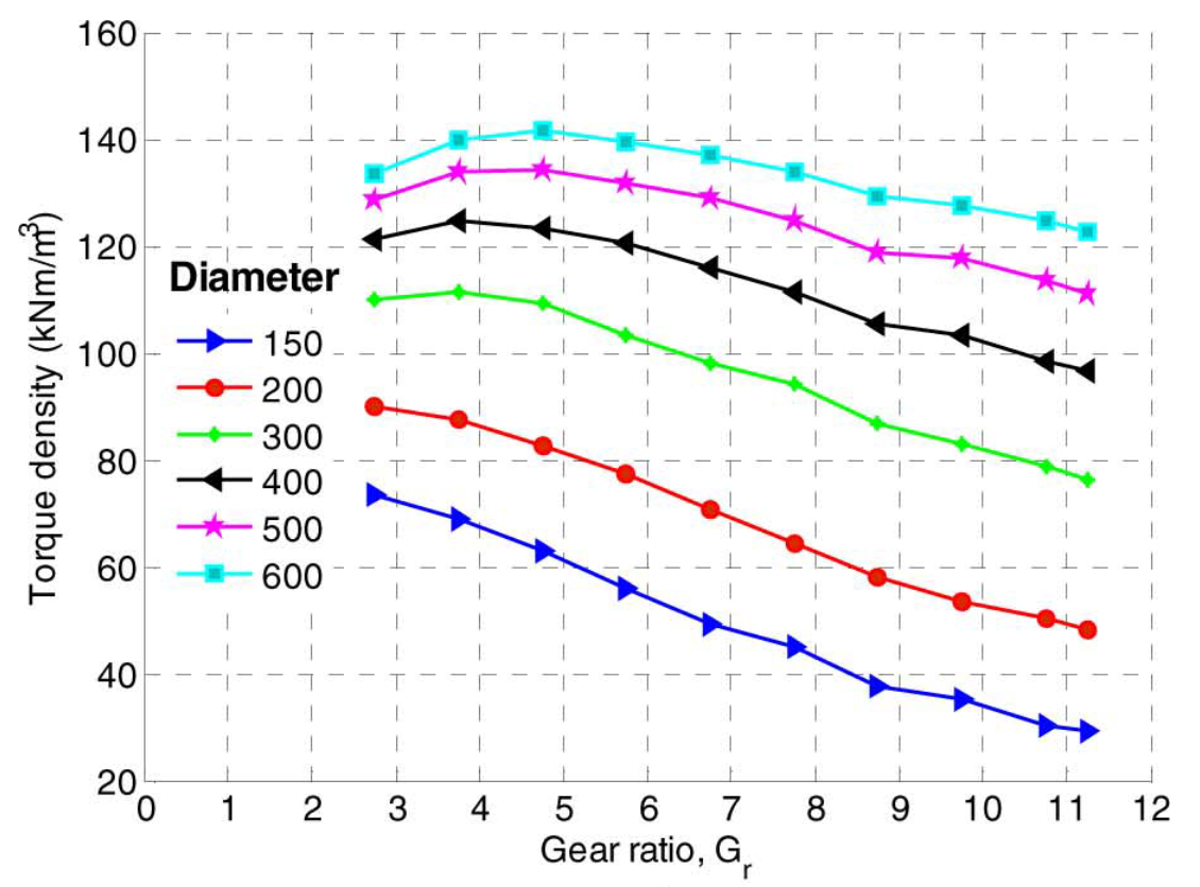
\includegraphics[width=0.45\textwidth]{torque_density_mag.png}
    \centering
    \caption[Hustota momentu síly referenčních magnetických převodovek]{Hustota momentu síly referenčních magnetických převodovek (zdroj: \cite{torque_dens}).}
    \label{fig:torque_density_mag}

    \vspace{1cm}

    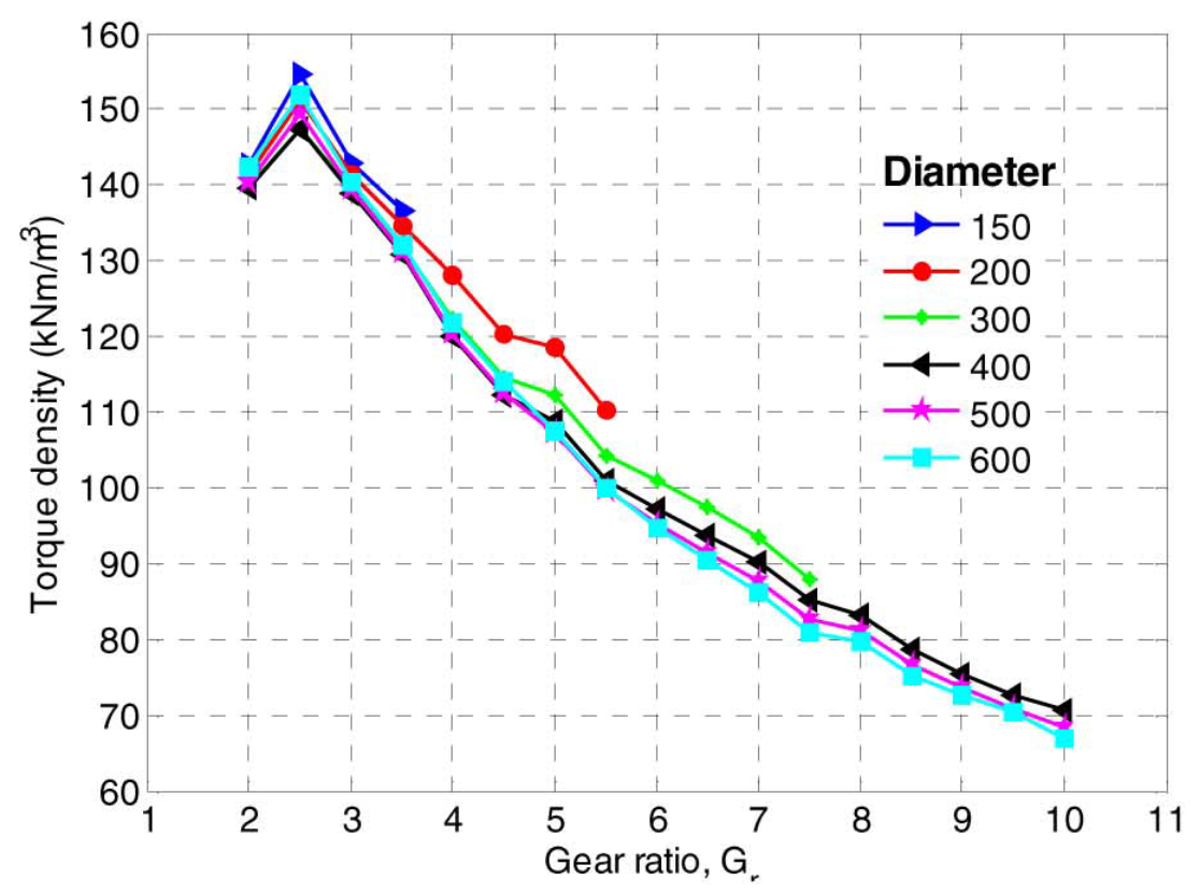
\includegraphics[width=0.45\textwidth]{torque_density_mech.png}
    \centering
    \caption[Hustota momentu síly referenčních mechanických převodovek]{Hustota momentu síly referenčních mechanických převodovek (zdroj: \cite{torque_dens}).}
    \label{fig:torque_density_mech}
\end{wrapfigure}

\subsection{Kompaktnost}
Dříve zmíněná kompaktnost magnetických převodovek spočívá ve spojení funkcí spojky, převodovky a momentového omezovače v jednom. Posouváním modulátoru po délce převodovky, která je rozdělena na 6 částí s různým počtem pólových párů, jsme schopni vybírat převod. Zároveň s tím magnety plní funkci spojky a momentového omezovače, protože při překonání maximálního momentu síly kolem sebe prostě proklouznou a znovu se zapojí až na dalším "magnetickém zubu". Návrh takové převodovky je k vidění na obrázku \ref{fig:magnetic_transmission}.

\subsection{Hustota momentu síly}
K porovnávání kvality převodovek je často používána míra momentu síly, který dokáže daný návrh přenášet, v závislosti na jejich objemu nebo hmotnosti. Při dopravě zařízení do vesmíru může právě objem nebo hmotnost hrát klíčovou roli v tom, zda bude zařízení použito. V grafech \ref{fig:torque_density_mag} a \ref{fig:torque_density_mech} je vidět porovnání hustot momentu síly magnetických a mechanických převodovek v závislosti na jejich průměru a převodovém poměru.

\subsection{Druhy magnetických převodů}
Princip magnetických převodů vychází ze schopnosti vytvořit pomyslný "magnetický zub", který nahrazuje klasické zuby v ozubených kolech. Rapidní vývoj silnějších a odolnějších magnetických látek dovoluje vytvářet nejrůznější konfigurace magnetických převodů a inspirovat se jejich mechanickými protějšky. Na obrázku \ref{fig:topologies_simple} jsou k vidění různé topologie magnetických převodů a jim odpovídajících mechanických ekvivalentů.
\begin{wrapfigure}{r}{0.50\textwidth}
    \vspace{-5cm}
    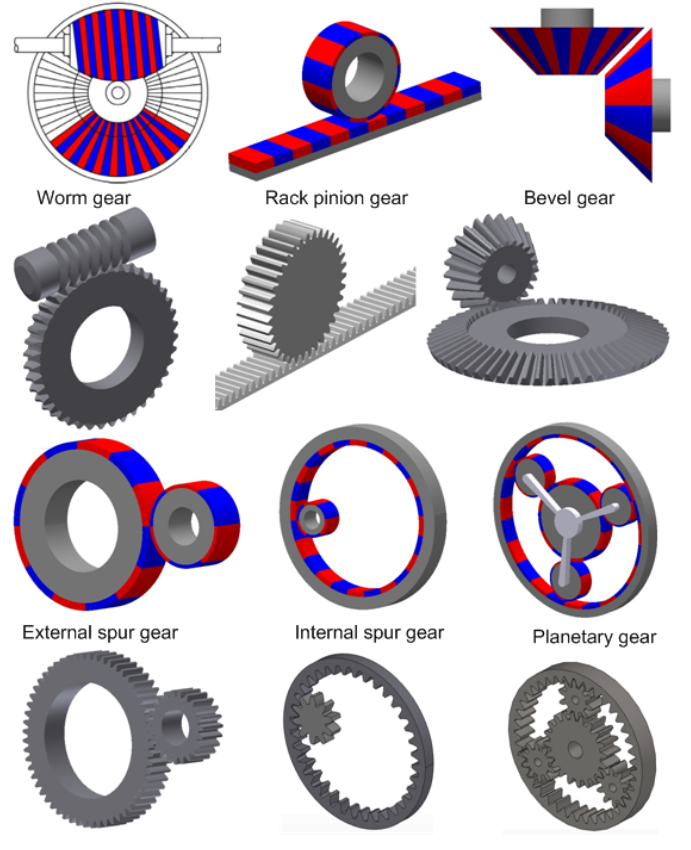
\includegraphics[width=0.45\textwidth]{simple_gears.png}
    \centering
    \caption{Základní magnetické topologie a jejich mechanické ekvivalenty (zdroj: \cite{MG_topologies}).}
    \label{fig:topologies_simple}
\end{wrapfigure}

Více pozornosti je však věnováno hlavně převodovkám s vyšší momentovou hustotou (planetární a harmonické) nebo jinou složitější topologií (koncentrické) (viz \autoref{fig:topologies_complex}).

Kromě topologie je také zájmem zkoumání orientace jednotlivých magnetů. Zde je dobré zmínit orientaci zvanou Halbachovo pole\footnote{Halbachovo pole (anglicky \textit{"Halbach array"}) je speciální uspořádání, jehož planární varianta se snaží o minimalizaci unikajícího pole z jedné strany.}.
\begin{figure}[H]
    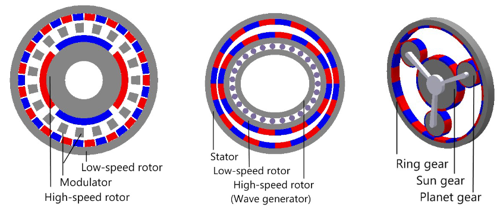
\includegraphics[width=0.45\textwidth]{torqe_dense_gears.png}
    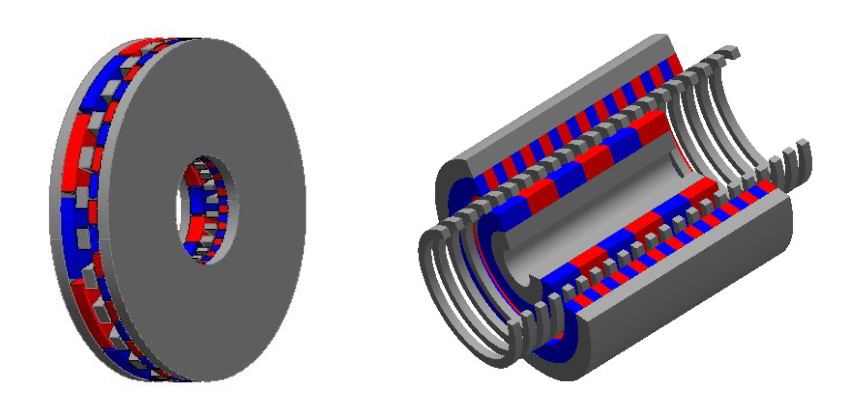
\includegraphics[width=0.45\textwidth]{concentric_gears.png}
    \centering
    \caption[Příklady magnetických převodů s vyšší hustotou momentu síly a koncentrických převodů]{Příklady magnetických převodů s vyšší hustotou momentu síly (první 3 zleva) a koncentrických převodů (první 2 zprava) (zdroj: \cite{MG_topologies}).}
    \label{fig:topologies_complex}
\end{figure}

\section{Vlastní návrhy}

\subsection{Princip fungování}

{
    \raggedright
    Námi vybraný způsob konstrukce převodovky odpovídá zleva prvnímu typu na obrázku \ref{fig:topologies_complex}. Tento systém je sestaven ze tří částí - vnějšího rotoru, vnitřního rotoru a modulátoru. Označíme-li počet magnetických párů vnějšího rotoru $p_{out}$, počet magnetických párů vnitřního rotoru $p_{in}$ a počet modulátorových násad $q_m$, jsme schopni v závislosti na tom, která část je stacionární, určit převodový poměr. Zároveň musíme splnit podmínku \cite{MG_topologies}, že $q_m = p_{in} + p_{out}$.
    V případě fixovaného vnějšího rotoru se převodový poměr $G_r$ počítá následovně\cite{MG_topologies}:
    \begin{equation}
        \label{eq:gear_ratio1}
        \begin{gathered}
            G_r = \frac{q_m}{p_{out}} = \frac{\omega_{out}}{\omega_{m}}
        \end{gathered}
    \end{equation}

    V případě fixovaného modulátoru se výpočt převodového poměru $G_r$ mění na \cite{MG_topologies}\footnote{Záporné znaménko u úhlových rychlostí v předchozí rovnici značí, že se vstup a výstup otáčejí opačným směrem.}:
    \begin{equation}
        \label{eq:gear_ratio1}
        \begin{gathered}
            G_r = \frac{p_{in}}{p_{out}} = -\frac{\omega_{out}}{\omega_{in}}
        \end{gathered}
    \end{equation}
}

Ústřední myšlenkou tohoto specifického návrhu je používání modulátoru, který, jak název napovídá, moduluje magnetické pole vnějšího rotoru. Účelem modulátoru je přeměna magnetické periody vnějšího rotoru na periodu vnitřního rotoru. Toho je docíleno tím, že modulátor a vnější rotor jsou mimo fázi (resp. počet pólových párů rotoru není stejný jako počet segmentů modulátoru). Pokud by byl počet stejný, každému magnetickému nástavci v modulátoru by připadal právě jeden magnet v vnějším rotoru a nástavce by tedy pouze kopírovaly magnetizace odpovídajících magnetů.

\begin{wrapfigure}{r}{0.50\textwidth}
    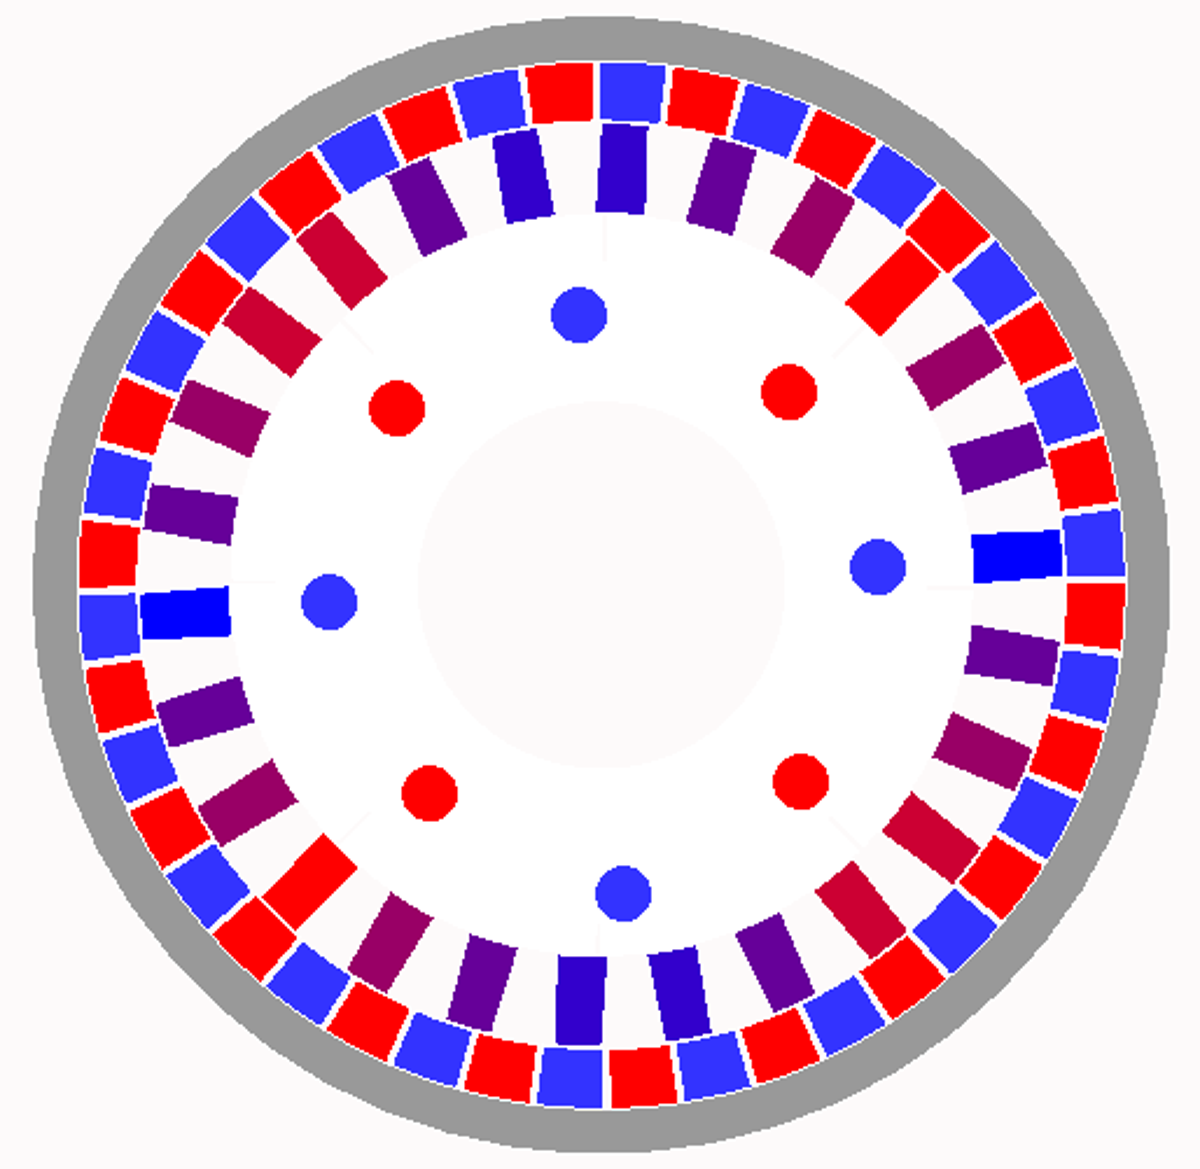
\includegraphics[width=0.45\textwidth]{modulation_explanation.png}
    \centering
    \caption[Ilustrace sčítání magnetizací na jednotlivých nástavcích modulátoru]{Ilustrace sčítání magnetizací na jednotlivých nástavcích modulátoru. Vnější rotor obsahuje 22 pólových párů. Modulátor je složen z 26 nástavců. Výsledná perioda je tedy $\frac{1}{4}.$}
    \label{fig:topologies_simple}
\end{wrapfigure}
Kdyby bylo v modulátoru o jeden nástavec více, existovala by vždy pouze jedna dvojice násady a magnetu, která by k sobě sedla perfektně. Všechny ostatní nástavce se pak nacházejí někde mezi magnety pólového páru. V tu chvíli se výsledná magnetizace na nástavci projevuje jako součet dvou nejbližších magnetizací magnetů. Tímto se v nástavcích modulátorů vytvoří magnetizační vlna o periodě 1, jelikož každý nástavec modulátoru je v lehce jiné relativní pozici vůči jeho nejbližším magnetům.

Zvedneme-li rozdíl $q_m$ a $p_{out}$ na dva, objeví se vlna o periodě $\frac{1}{2}$. Navyšujeme-li rozdíl, je pokračování tohoto chování zřejmé. Díky tomuto principu platí i podmínka $q_m = p_{in} + p_{out}$, protože perioda vnitřního rotoru musí odpovídat modulované periodě.

\subsection{První návrh}

Náš první návrh využívá 12 pólových párů ve vnějším a 4 pólové páry ve vnitřním rotoru. Celkový počet modulátorových násad je tedy 16 a ty jsou tvořeny železnými válci, které jsou získány nařezáním správně tlustých hřebíků.

Vnitřní rotor (viz \autoref{fig:MT_v1_inner}) je válcového tvaru s 8 výřezy na neodymové magnety rozměrů 3mm x 4mm x 20mm. V každém z výřezů je ze spodní strany udělána dírka, kterou je možné pomocí tenkého klíče magnety vysunout. Z horní a dolní podstavy rotoru vychází hřídel s šestiúhelníkovým výřezem určeným pro vložení klíče. Vnitřní rotor je z jedné strany zasazen do ložiska uvnitř modulátoru. Z druhé strany je držen ložiskem ve víku vnějšího rotoru.

\begin{wrapfigure}{r}{0.4\textwidth}
    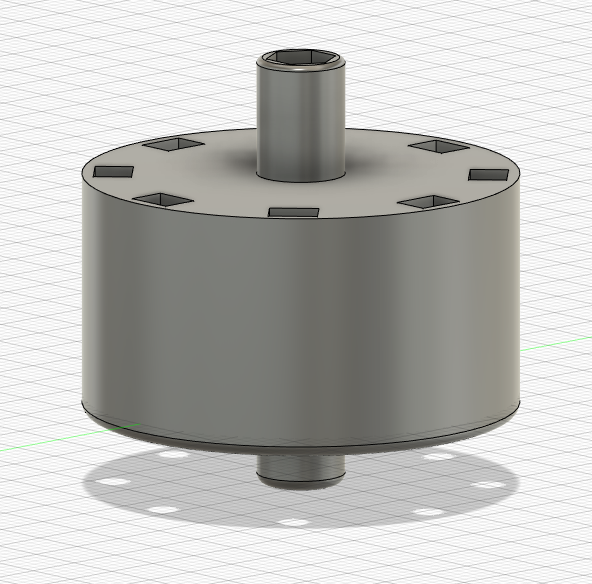
\includegraphics[width=0.35\textwidth]{MT_v1_inner.png}
    \centering
    \caption{Vnitřní rotor prvního návrhu převodovky}
    \label{fig:MT_v1_inner}

    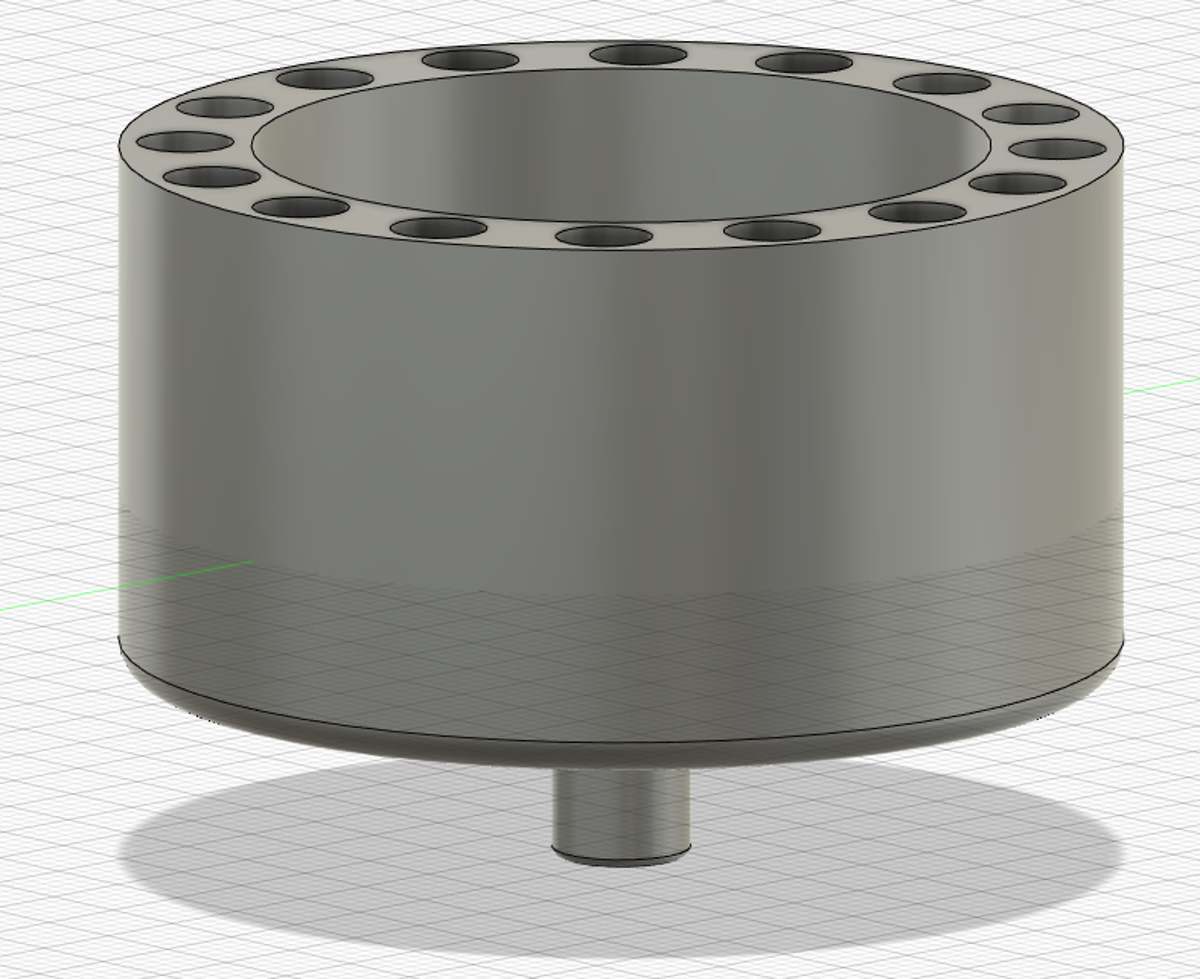
\includegraphics[width=0.35\textwidth]{MT_v1_modulator.png}
    \centering
    \caption{Modulátor prvního návrhu převodovky}
    \label{fig:MT_v1_modulator}

    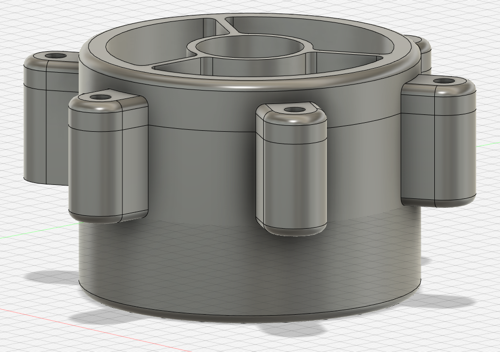
\includegraphics[width=0.35\textwidth]{MT_v1_outer.png}
    \centering
    \caption{Vnější rotor prvního návrhu převodovky}
    \label{fig:MT_v1_outer}
\end{wrapfigure}
Modulátor (viz \autoref{fig:MT_v1_modulator}) má tvar dutého válce a po jeho obvodu jsou vyříznuty válcové otvory pro magnetické násady. Z dolní strany je upevněn do ložiska, které je na spodní straně vnějšího rotoru. V dutině válce je umístěno ložisko, do kterého je vložen vnitřní rotor. Toto dovoluje nezávislý pohyb vnitřního rotoru a modulátoru.

Vnější rotor (viz \autoref{fig:MT_v1_outer}) je složen z dvou částí - těla a víka. Víko drží ložisko vnitřního rotoru, čímž mechanicky izoluje oba rotory. Tělo má 24 výřezů na magnety stejných rozměrů jako u vnitřního rotoru. Spodek těla je zakončen ložiskem, které izoluje modulátor od těla. Na této straně je výstupní hřídel modulátoru (opět s šestiúhelníkovou dírou na klíč). Zároveň jsou po stranách těla umístěny úchytné body určené k sešroubování těla a víka.

Všechny 4 součásti jsou poté vytvořeny pomocí 3D tisku a jsou do nich vsazeny ložiska, magnety a magnetické válce.

\begin{figure}[H]
    \raggedright
    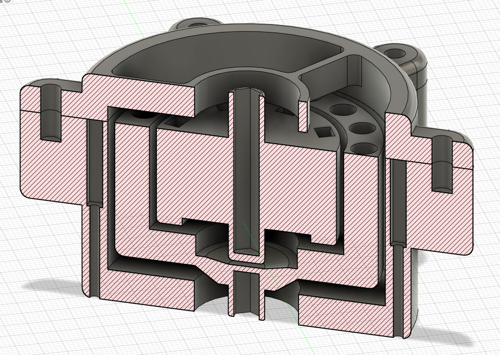
\includegraphics[width=0.5\textwidth]{MT_v1_whole_cut.png}
    \captionsetup{justification=raggedright,singlelinecheck=false}
    \caption{Řez celou magnetickou převodovkou.}
    \label{fig:MT_v1_whole_cut}
\end{figure}

\clearpage

\begin{wrapfigure}{r}{0.5\textwidth}
    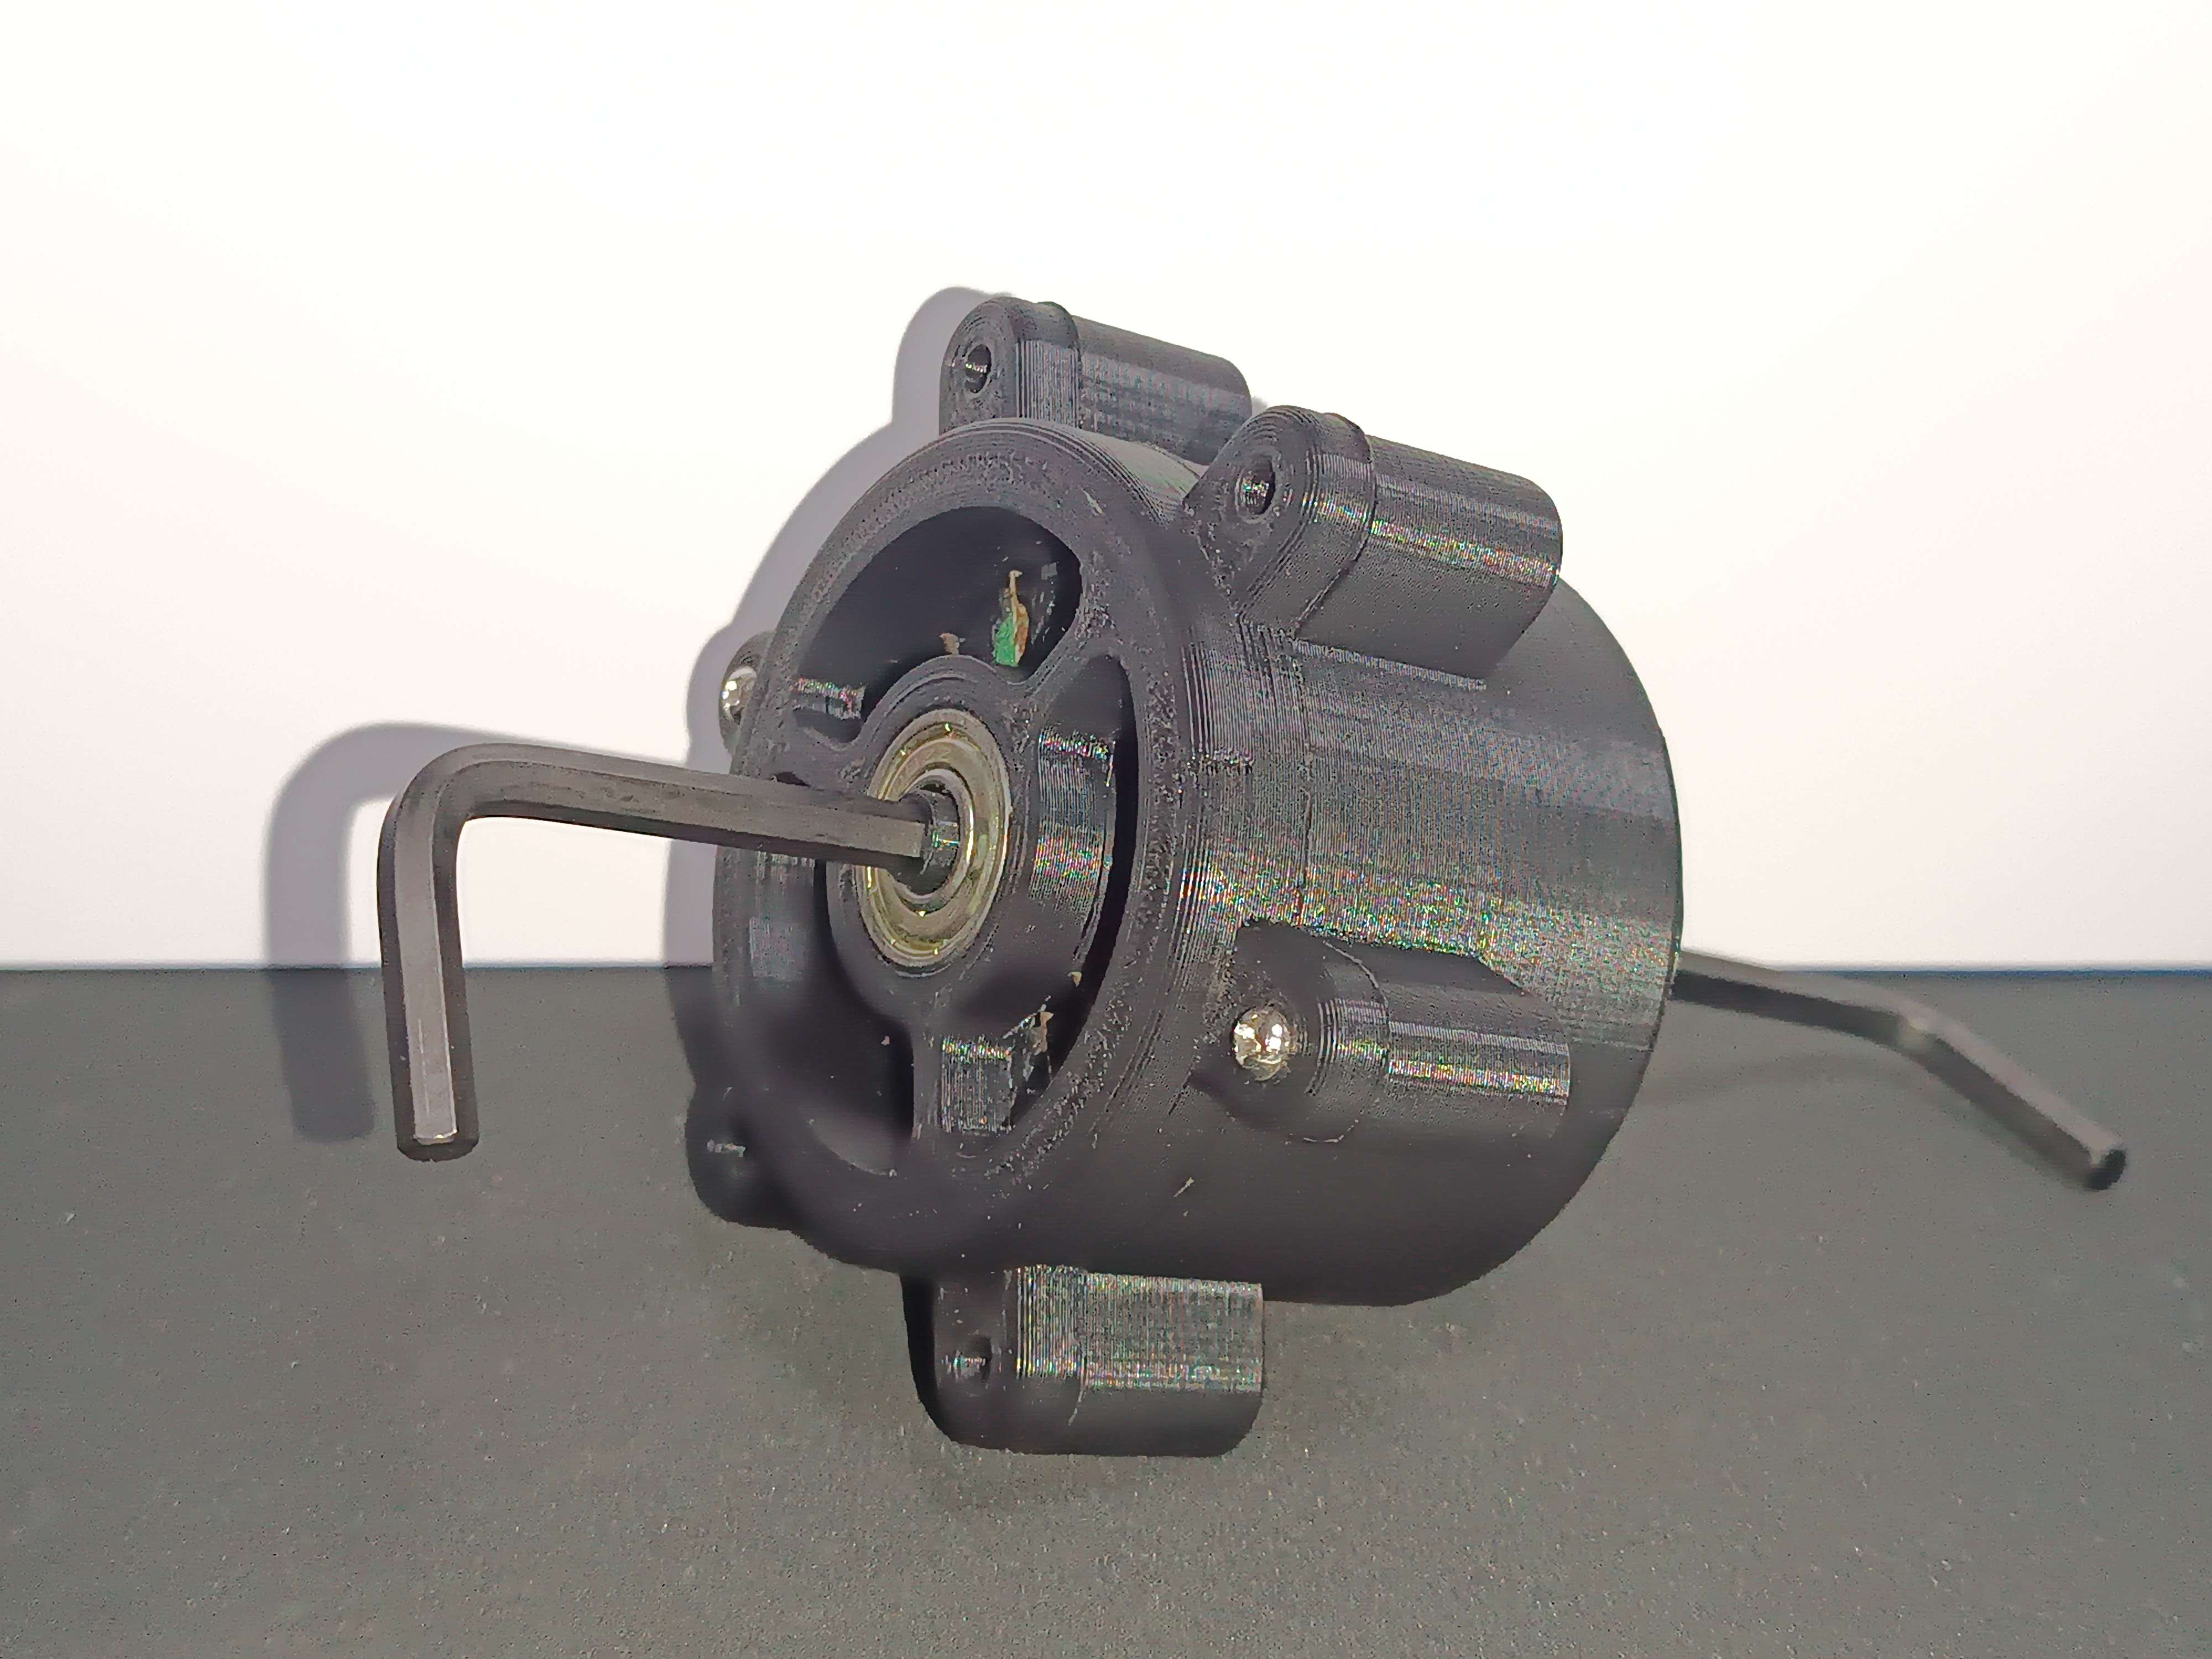
\includegraphics[width=0.45\textwidth]{MT_v1_photo.png}
    \centering
    \caption{Konstrukce první návrhu}
    \label{fig:MT_v1_inner}
\end{wrapfigure}
První prototyp převodovky byl po lehkých úpravách sice funkční, ale nepříliš uspokojivý. První chybou bylo použití kovových válců v modulátoru, které byly příliš blízko sebe a docházelo mezi nimi k "magnetickému zkratu". Po opravení tohoto problému vyměněním válců transformátorovými plechy již převodovka fungovala. Druhou zásadní chybou bylo, že magnety a modulátor byly příliš daleko od sebe. Šířka mezery mezi modulátorem a rotory byla 3mm a tloušťka stěn rotorů tvořila mezeru další 2mm. Toto byl jeden z hlavních důvodů, proč převodovka nebyla příliš silná, protože magnetická síla klesá se čtvrtou mocninou. Posledním problémem bylo, že modulátor je upevněn pouze v jednom bodě a to ve spodním ložisku. Toto ložisko není perfektní a modulátor se působením magnetů naklání ke vnitřním stranám vnějšího rotoru.

Motivace opravit tyto chyby a vylepšit návrh tedy vedla k druhé iteraci.

\subsection{Druhý návrh}

\begin{wrapfigure}{r}{0.4\textwidth}
    \vspace{-2.5cm}
    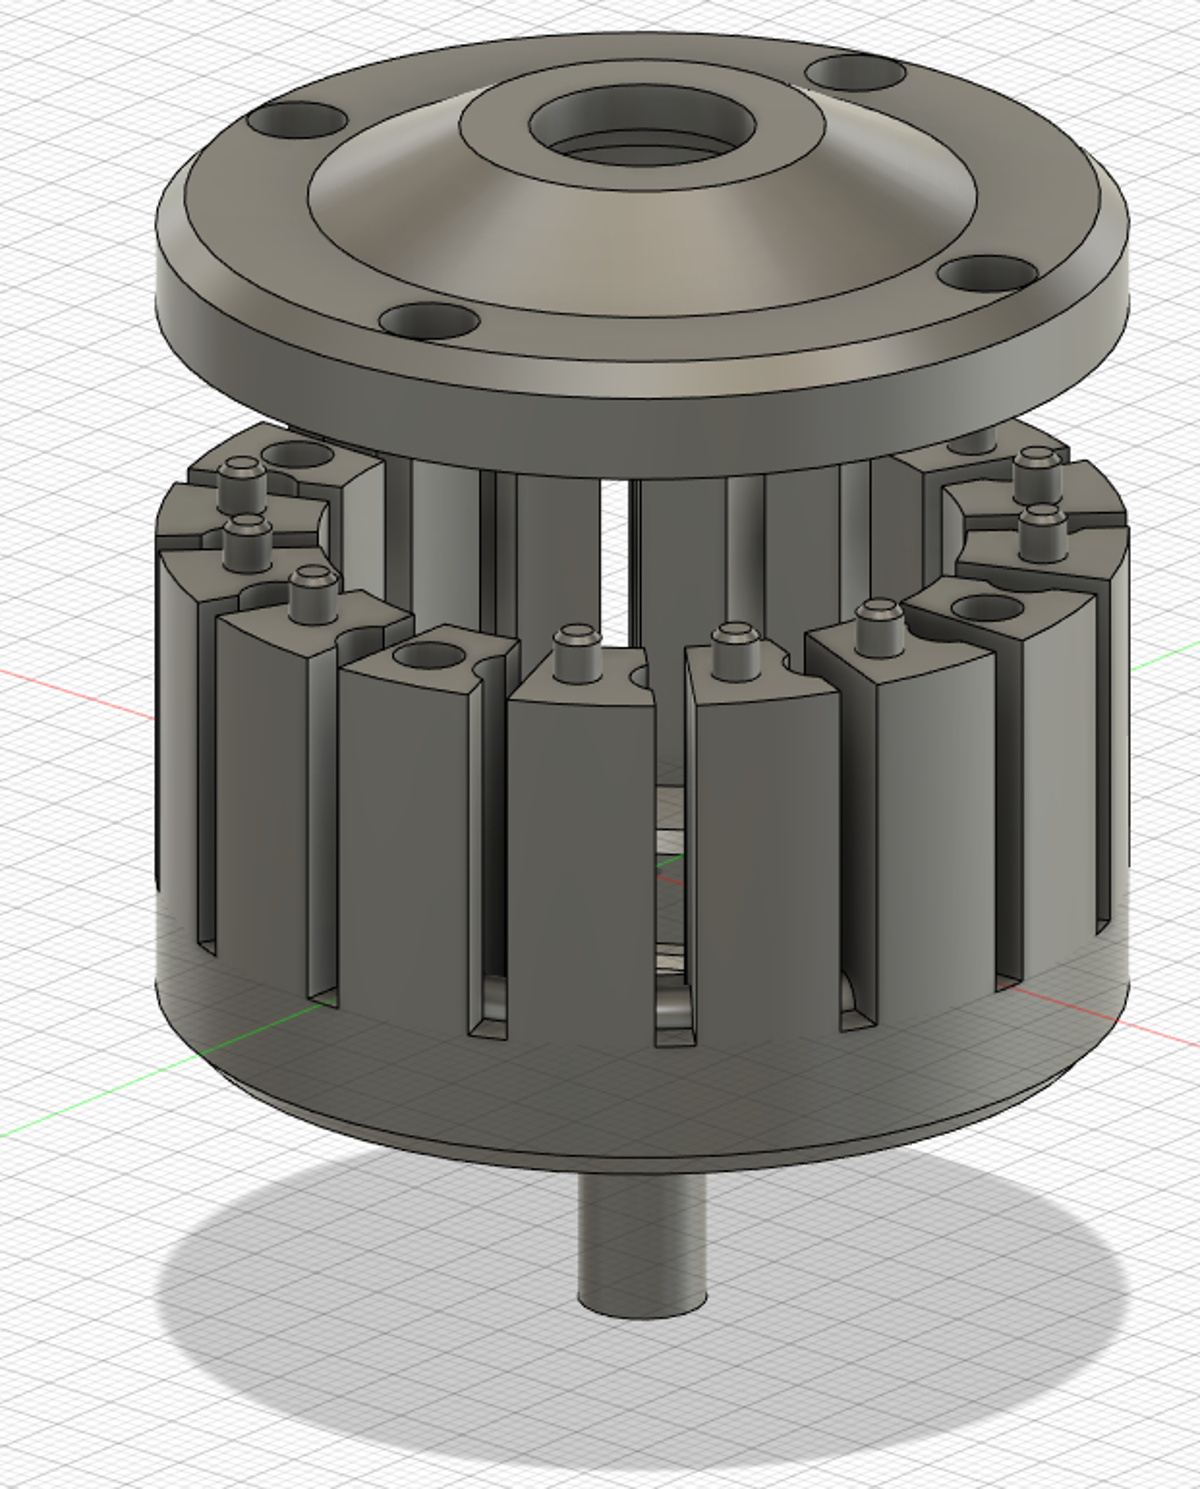
\includegraphics[width=0.3\textwidth]{MT_v2_modulator.png}
    \centering
    \caption{Modulátor druhého návrhu převodovky}
    \label{fig:MT_v2_modulator}

    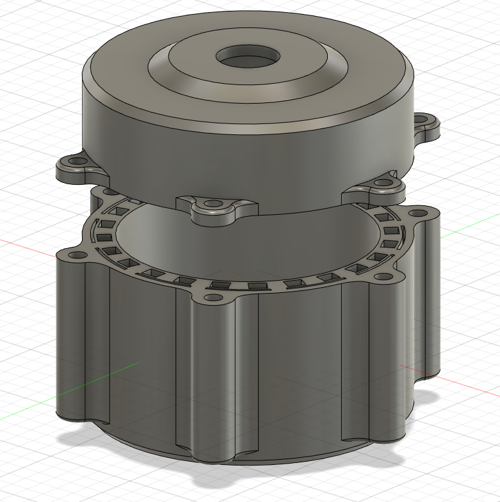
\includegraphics[width=0.3\textwidth]{MT_v2_outer.png}
    \centering
    \caption{Vnější rotor druhého návrhu převodovky}
    \label{fig:MT_v2_outer}
\end{wrapfigure}
Druhý návrh převodovky je stejného typu a používá stejný počet magnetů v jeho jednotlivých částech. Vnitřní rotor je velmi podobný původnímu rotoru (je pouze lehce zvětšen), a proto ho nebudeme znovu popisovat. 

Modulátor (viz \autoref{fig:MT_v2_modulator}) je v tomto případě stavěn tak, aby do něj byly vloženy plechy místo válců. Každá z 16 přihrádek může objímat až 5 plechů tloušťky 0.5mm. Variabilní počet plechů dovolujeme, jelikož se chceme v budoucnu zabývat tím, jaký má tloušťka násady dopad. Druhou novinkou je, že modulátor má své vlastní víko, ve kterém drží vnitřní rotor. Toto je druhý záchytný bod modulátoru, který v předchozím návrhu chyběl.

Vnější rotor (viz \autoref{fig:MT_v2_outer}) je velmi podobný původnímu rotoru, pouze lehce větší. Dále jsou do něj připraveny škvíry, do kterých bude umístěn plech, který bude stínit magnetické pole vnějších magnetů.

\clearpage
{
    Všech pět dílů je opět vytisknuto na 3D tiskárně. 
    \raggedright
    Po nařezání plechů laserovou řezačkou jsou umístěny do určených přihrádek a nakonec jsou doplněny magnety a ložiska, čímž získáváme celou magnetickou převodovku (viz \autoref{fig:MT_v2}).
}

\begin{figure}[H]
    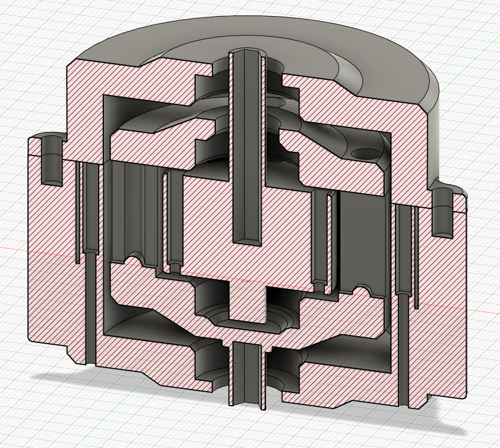
\includegraphics[width=0.45\textwidth]{MT_v2_whole_cut.png}
    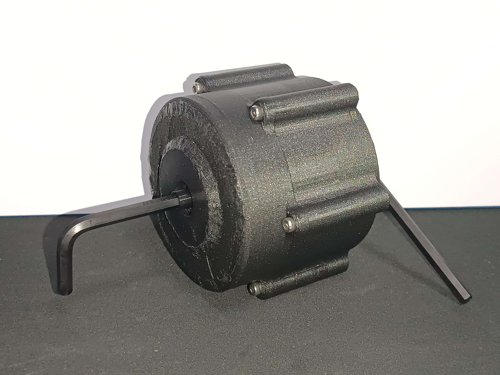
\includegraphics[width=0.45\textwidth]{MT_v2_photo.png}
    \centering
    \caption{Řez a fotografie finálního návrhu druhé převodovky.}
    \label{fig:MT_v2}
\end{figure}


% \subsection{Měření}
% Měření plechů